%You can leave alone everything before Line 79.
\documentclass{article}
\usepackage{url,amsfonts, amsmath, amssymb, amsthm,color, enumerate}
\usepackage{fullpage}
\usepackage{subfigure}
\usepackage{graphicx}
% Page layout
%\setlength{\textheight}{8.75in}
%\setlength{\columnsep}{2.0pc}
%\setlength{\textwidth}{6.5in}
%\setlength{\topmargin}{0in}
%\setlength{\headheight}{0.0in}
%\setlength{\headsep}{0.0in}
%\setlength{\oddsidemargin}{0in}
%\setlength{\evensidemargin}{0in}
%\setlength{\parindent}{1pc}
\newcommand{\shortbar}{\begin{center}\rule{5ex}{0.1pt}\end{center}}
\newcommand{\xxx}[1]{\textcolor{red}{#1}}
%\renewcommand{\baselinestretch}{1.1}
% Macros for course info
\newcommand{\courseNumber}{EECS 545}
\newcommand{\courseTitle}{Machine Learning}
\newcommand{\semester}{Winter 2012}
% Theorem-like structures are numbered within SECTION units
\theoremstyle{plain}
\newtheorem{theorem}{Theorem}[section]
\newtheorem{lemma}[theorem]{Lemma}
\newtheorem{corollary}[theorem]{Corollary}
\newtheorem{proposition}[theorem]{Proposition}
\newtheorem{statement}[theorem]{Statement}
\newtheorem{conjecture}[theorem]{Conjecture}
\newtheorem{fact}{Fact}
%definition style
\theoremstyle{definition}
\newtheorem{definition}[theorem]{Definition}
\newtheorem{example}{Example}
\newtheorem{problem}[theorem]{Problem}
\newtheorem{exercise}{Exercise}
\newtheorem{algorithm}{Algorithm}
%remark style
\theoremstyle{remark}
\newtheorem{remark}[theorem]{Remark}
\newtheorem{reduction}[theorem]{Reduction}
%\newtheorem{question}[theorem]{Question}
\newtheorem{question}{Question}
%\newtheorem{claim}[theorem]{Claim}
%
% Proof-making commands and environments
\newcommand{\beginproof}{\medskip\noindent{\bf Proof.~}}
\newcommand{\beginproofof}[1]{\medskip\noindent{\bf Proof of #1.~}}
\newcommand{\finishproof}{\hspace{0.2ex}\rule{1ex}{1ex}}
\newenvironment{solution}[1]{\medskip\noindent{\bf Problem #1.~}}{\shortbar}

%====header======
\newcommand{\solutions}[4]{
%\renewcommand{\thetheorem}{{#2}.\arabic{theorem}}
\vspace{-2ex}
\begin{center}
{\small  \courseNumber, \courseTitle
\hfill {\Large \bf {#1} }\\
\semester, University of Michigan, Ann Arbor \hfill
{\em Date: #3}}\\
\vspace{-1ex}
\hrulefill\\
\vspace{4ex}
{\normalsize Project Report}\\
{\LARGE  #2}\\
\vspace{2ex}
\end{center}
\begin{trivlist}
\item \textsc{Team members:} {#4}
\end{trivlist}
\noindent
\vspace{-1cm}
\shortbar
\vspace{-0.5cm}
}
% math macros
\newcommand{\defeq}{\stackrel{\textrm{def}}{=}}
\newcommand{\Prob}{\textrm{Prob}}
%==
\usepackage{graphicx}
\begin{document}
%%%%%%%%%%%%%%%%%%%%%%%%%%%%%%%%%%%%%%%%%%%%%%%%%
%\solutions{Your name}{Problem Set Number}{Date of preparation}{Collaborators}{Prover}{Verifiers}
\solutions{}{Coping with Complex Games using Machine Learning}{\today}{\\ Keegan R. Kinkade, @kinkadek\\ Pedro d'Aquino, @pdaquino \\Shiva Ghose, @gshiva }
%%%%%%%%%%%%%%%%%%%%%%%%%%%%%%%%%%%%%%%%%%%%%%%%%
%\renewcommand{\theproblem}{\arabic{problem}} 
%%%%%%%%%%%%%%%%%%%%%%%%%%%%%%%%%%%%%%%%%%%%%%%%%
%
% Begin the solution for each problem by
% \begin{solution}{Problem Number} and ends it with \end{solution}
%
% the solution for Problem 

\begin{abstract}
Robocode\cite{robocode} is a battle-tank simulator in which agents battle against each other in a dynamic environment. Traditionally, most agents have been hand-coded. In this project, we create an agent that utilizes machine learning techniques to decide which actions to take. In particular, we use support vector machines to learn evasion and targeting strategies, achieving competitive results. We also implement Q-learning to learn targeting strategies, but with less success. We test our robot against available competitive Robocode agents and present our results.
\end{abstract}

\section{Introduction}

Initially released in 2001 with the aim of assisting in learning object oriented programming, Robocode is an open source, dynamic, deterministic tank battling simulator implemented in Java. Each Robocode agent is designed to control a virtual differentially-driven tank, equipped with mounted rotating gun turret and enemy scanning radar, in order to attack enemy tanks with similar features but opposing strategies. While the environment has made it simple to create an agent capable of moving, targeting, and shooting, perfecting agents to do well against multiple opponent strategies has proven to be difficult. There has been research to optimize agents using both neural networks as well as genetic programming. However, little work has been done to incorporate sophisticated machine learning techniques designed to better inform Robocode agents when making decisions. 

\subsection*{Statement of the Problem}

Succeeding in Robocode battles requires an agent that is capable of predicting an opponent's actions in order to optimize its performance. The purpose of this project is to incorporate machine learning algorithms in a Robocode agent in order to assist the decision making process while attempting to defeat opponents. Specifically, we focus on incorporating machine learning in two areas: \emph{evasion} and \emph{targeting}. To simplify the models, we consider these areas separately. With respect to evasion, our goal is to evade incoming bullets in order to minimize the damage inflicted by opponents. Conversely, the goal is to fire bullets in a manner that maximizes the damage inflicted upon opponents. To this end, we aimed to create agents that learn how to evade and target effectively, measuring the overall performance by competing against human-written agents. 

 
\section{Review of Related Work}
Robocode has provided a powerful base upon which artificial intelligence methods can built up, taught and tested. This aspect of Robocode was explored as early as 2004\cite{Hartness}. Over the years various approaches have been used to develop highly competitive robots in this platform. The most successful so far have been systems built up on hand tuned heuristics which are aided by statistical methods. 

The majority of the research work done in this environment has been towards the application of Genetic Algorithms in evolving agents rather than evolving strategies\cite{strategies, gp1, gp2}.  Shichel et al.\cite{gp1}, used genetic programming to evolve tank strategies for a robot in the HaikuBot category (which allows robots whose code is no longer than 4 lines). They evolved a population of 256 robots over approximately 400 generations. Their robot was ranked 3rd in the HaikuBot category. Woolley et al.\cite{woolley} discuss the implementation of a hybrid reactive robot control system and use Robocode as a platform to verify their claims. Their work focuses on the ability of their system to mimic existing reactive control architectures. Reinforcement learning has also been used in Robocode to develop movement strategies for agents\cite{gade}. Other researchers have looked into using Neuro-Evolutionary methods with Augmented Topologies (NEAT) and Artificial Neural Networks (ANNs)\cite{nielsenAI} to control the targeting systems.

In one of the very few academic mentions of Robocode outside of the artificial intelligence field, Kobayashi et al. make a study of various sets of targeting strategies employed in Robocode\cite{strategies}. However they do not explicitly state any methods to calculate the expected utilities of employing each strategy given a scenario.

Overall, the work we present in this paper presents a novel implementation of a combination of support vector machines and reinforcement learning methods to design an agent capable of competing with the top most agents in Robocode.

\section{Experimental Methodology}
In this section, we describe the methods used to learn evasion and targeting strategies. Throughout the project, evasion and targeting were treated as two independent areas. This assumption is valid because the actions of the gun turret can be decoupled from the movement platform. To evade a bullet, we have the agent choose one evasion movement from a predetermined set. Targeting was implemented in two different approaches: the first was similar to evasion in that an agent had a subset of actions to choose from, while the second method explored the use of reinforcement learning.

\subsubsection*{General Movement}
The default behavior of the agent is to closely mirror the behavior of the opponent while keeping a set distance from it. In general the probability of getting hit by incoming fire is inversely proportional to how close the observer is to the firing point. We want the agent to move closer to the enemy when it has higher health to maximize the probability of hitting the enemy and to stay further back when it has lower health to better evade incoming fire. This was modeled as series of attracting and repelling force interactions.

\subsection*{Evasion}
When the opponent fires at the evasion agent, the mirroring behavior is suppressed and a random evasion movement is chosen. For training, we designed the system to choose a random movement so that the agent would explore the entire space of possible evasions. Four simple evasion movements were designed based on watching many battles of other agents and detecting patterns in the way that expertly-written robots behaved.

\paragraph{Dodge Left/Right:}
In these two evasion movements, the agent moves to the left or right of the opponent when it is fired upon. This movement strategy is represented in Figure \ref{LR}, where $\Psi$ is the relative bearing to the opponent ($-180^{\circ} \leq \Psi \leq 180^{\circ}$). There are two different turning cases for $\Psi$: one when the agent is facing direction $d_1$ corresponding to bearing $\Psi_1$, and second when the agent is facing direction $d_2$ corresponding to bearing $\Psi_2$. Because we have a differential driven robot, we desire to turn a minimum distance to position our drive track perpendicular to the line of sight between us and the opponent. Achieving this angle is done in tandem with moving either forward or backward depending on whether we are dodging left or right.

\begin{figure}[t]
\begin{minipage}[b]{0.5\linewidth}
	\centering
		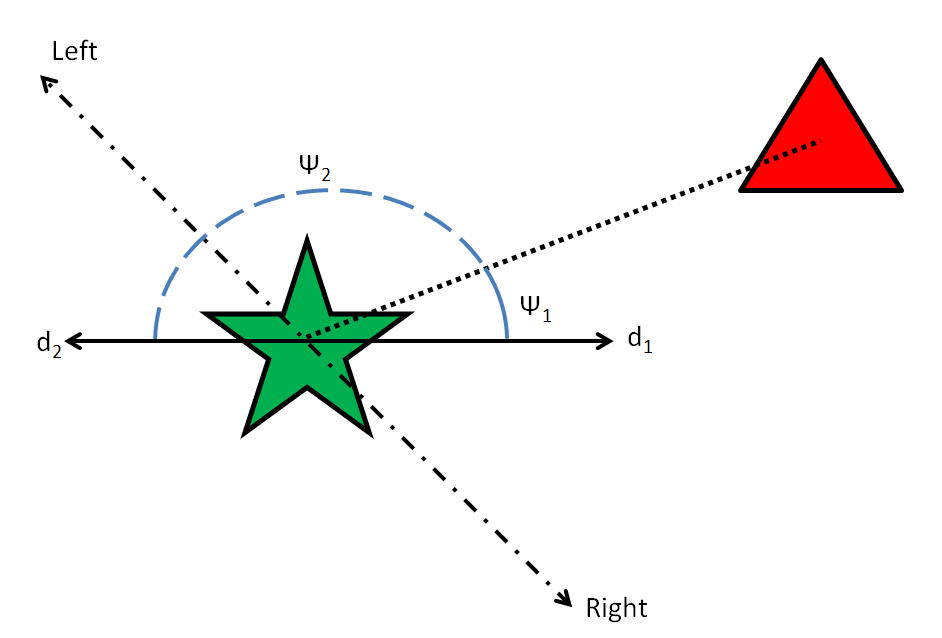
\includegraphics[width=6 cm]{LR}
	\caption{Left--Right dodging strategy.}
	\label{LR}
\end{minipage}
\hspace{0.5cm}
\begin{minipage}[b]{0.5\linewidth}
	\centering
		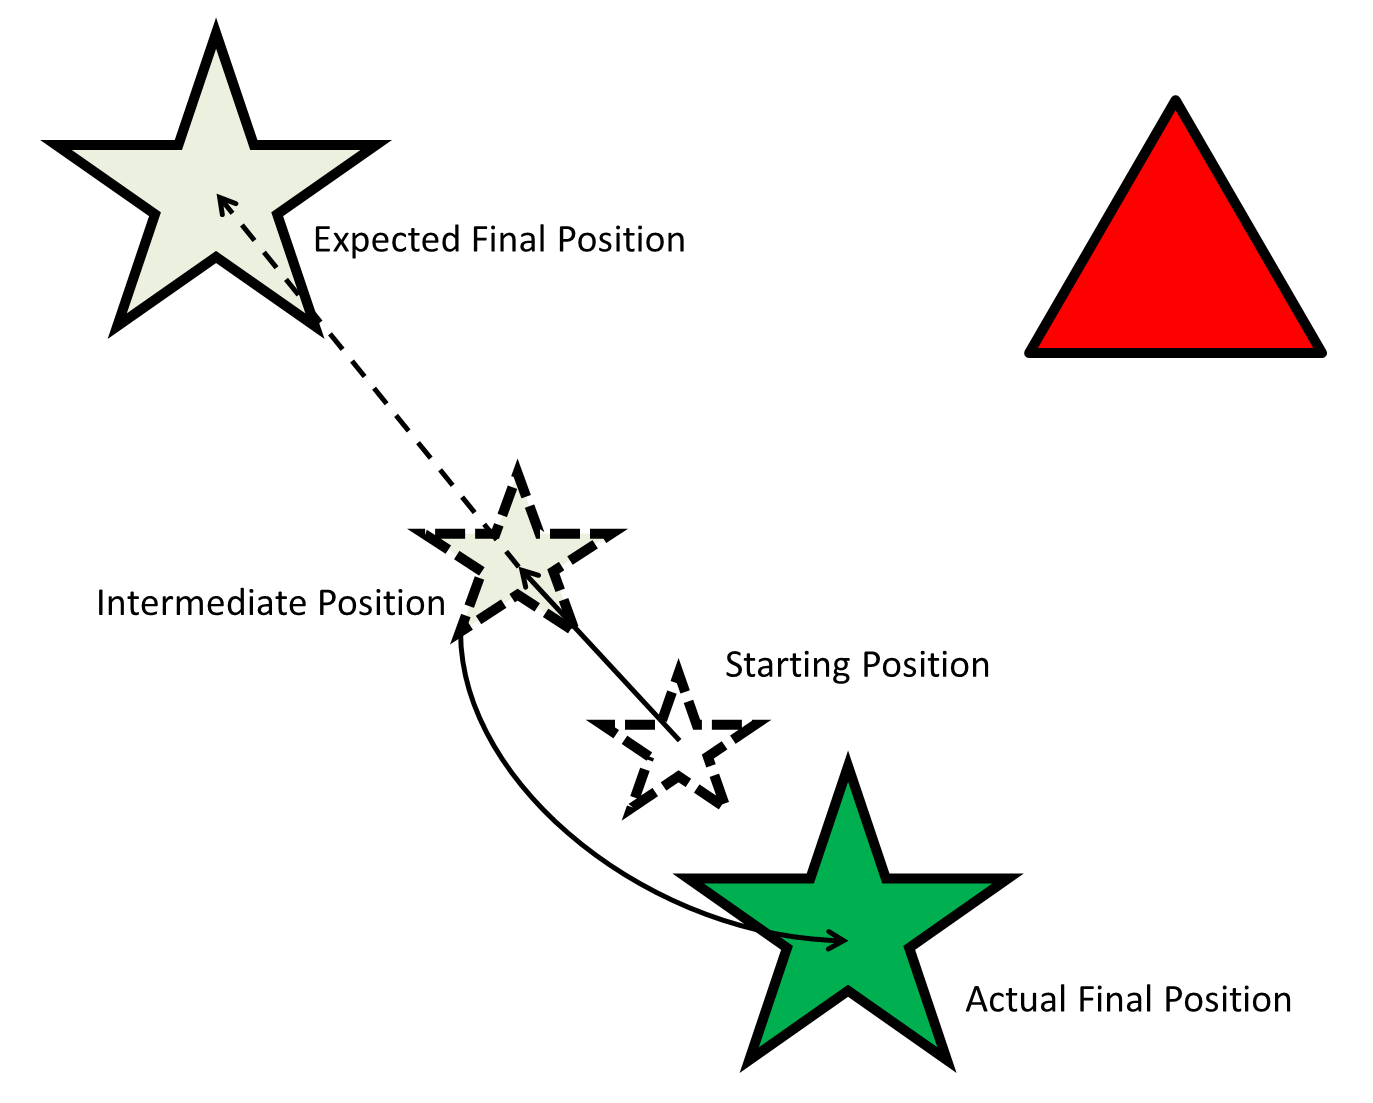
\includegraphics[width=6 cm]{Feign.png}
	\caption{Feigning}
	\label{feign}
\end{minipage}
\end{figure}

\paragraph{Feign:}
When feigning, the agent immediately reverses its direction of motion (Robocode allows for full speed both backwards and forwards). This movement is illustrated in Figure \ref{feign}.

\paragraph{Halt:}
Halting is simply stopping movement. This is useful against robots that assume the opponent will continue moving in a particular directions after it has been fired upon.

\subsubsection*{Learning the Evasion Strategy}
In order to learn which evasion movement the agent should employ when fired upon, an SVM for each movement was trained\footnote{We also experimented with using one single SVM and considering the movement employed as a feature, but the performance was degraded.}. Each SVM was trained to predict whether employing the evasion movement at a given state would result in the agent dodging the bullet (+1) or being hit (-1). At its essence, we are testing the ability of the agent to stay alive, but with the simplifying assumption that bullets are independent (i.e. dodging a bullet is always good, regardless of the new state the agent goes to).
 
The following features were used to represent the state of the battlefield:

\begin{itemize}
	\item global position and velocity of the agent in $x$, $y$ and $\theta$ (its bearing)
	\item the global and relative (with respect to the agent) positions  and velocities of the opponent, in $x$, $y$ and $\theta$
	\item the distance and bearing between the agent and the center of the battlefield
	\item the Euclidian distance between the agent and the opponent
	\item the health of the agent and of the opponent
\end{itemize}

These features were heuristically selected. After we collected enough data, we ran F-score based tests\cite{Chen05combiningsvms} to reduce the feature set, but no performance gain could be achieved by using less features.

In order to train the SVMs, labels were provided that expressed if the evasion strategy employed was effective at dodging a bullet. To do so, bullets fired by opponents had to be tracked. This, in general, is not a straightforward task in Robocode, as the agent cannot sense the position of a bullet using its radar. However, in order to fire a bullet, a tank must sacrifice some of its own energy. The radar-sensor can detect such a drop in energy of the opponent. Using the detection of an energy drop, we were able to determine when the enemy had fired a bullet and track it as a wave propagation, as depicted in Figure \ref{b_wave}. When the agent detects that the bullet wave has passed its location, the evasion movement is considered to have been successful. One consequence of this modeling approach is that the agent is only able to learn how to evade one bullet at a time. Subsequent bullets fired while the agent is already tracking a previous bullet are ignored.

\begin{figure}[t]
\begin{minipage}[b]{0.5\linewidth}
	\centering
		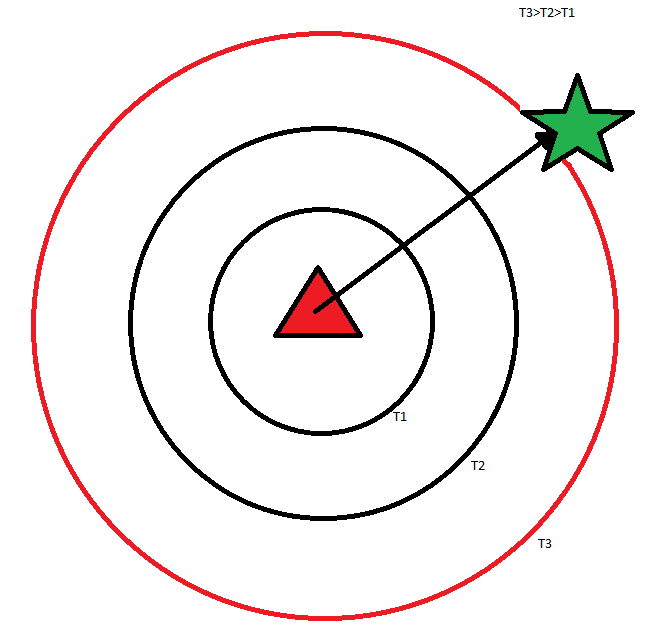
\includegraphics[width=5 cm]{bullet_wave.png}
	\caption{Bullet waves at different time steps.}
	\label{b_wave}
\end{minipage}
\hspace{0.5cm}
\begin{minipage}[b]{0.5\linewidth}
\centering
		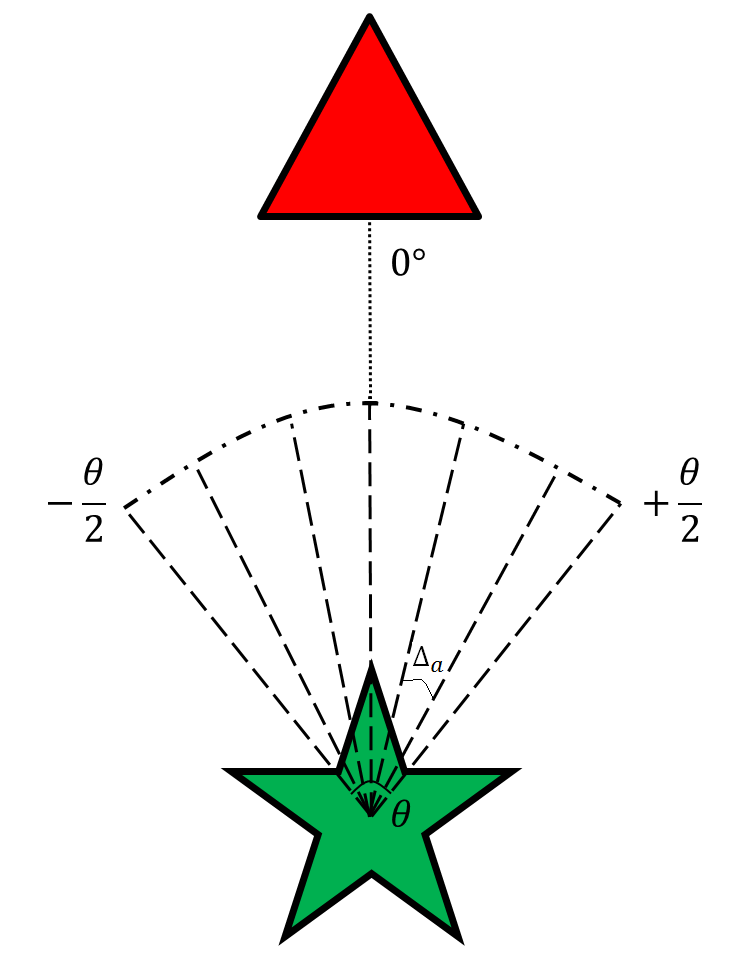
\includegraphics[width=5 cm]{targeting.png}
	\caption{Discretization of targeting solutions.}
	\label{tget}
\end{minipage}
\end{figure}

\subsection*{Targeting Strategies}
The objective of a targeting agent is to predict where the opponent will be in the future and shoot according to that prediction. The values that the firing angle can take are continuos over the interval $[0^{\circ}, 360^{\circ}]$. Thus, in order to make calculations tractable, the operating region was discretized between $[-\frac{\theta}{2}, +\frac{\theta}{2}]$, where $\theta$ is the firing arc range and $0^{\circ}$ represents head on alignment with the opponent.

\subsubsection*{SVM}
After successfully implementing SVMs for evasion purposes, an SVM was used to predict the best firing angle. This not only allowed the agent to successfully target the enemy, but also served as a benchmark for the application of Q-learning for targeting. Whereas multiple SVMs were trained for individual evasion strategies, a single SVM was used for targeting by treating the firing angle as an additional feature to those presented earlier. The firing angle was limited to $[-40^{\circ}, 40^{\circ}]$ ($\theta = 80^{\circ}$) and discretized into 21 angles, each separated by $\Delta_a = 2^{\circ}$. A firing arc range of $80^{\circ}$ ensures that the enemy agent is unable to outrun a fired shot based on the dimensions and physics of the environment. Furthermore, the discretization ensures that when used to target the enemy, only 21 different prediction calls (one for each possible firing angle) will be made to the SVM, reducing the overall decision making time required by the agent.

Data for the targeting SVM was collected by having an agent pick a firing angle at random and firing bullets according to that firing angle. Bullet tracking for providing labels in targeting is simplified by the Robocode environment as it provides full detailed information to agents about their own fired bullets. Labels for targeting are added to training data points according to whether the bullet hits the enemy (+1) or misses and leaves the environment (-1). When determining how to fire using this targeting SVM, predictions must be made using the current features of the state with each possible firing angle. The same features were used as those in the evasion SVMs.

\subsubsection*{Q-learning}
Q-learning \cite{watkins92a} is a method to learn a function $Q(s, a)$ that attributes an utility value to taking an action $a$ at state $s$. This method has two interesting properties among other reinforcement learning algorithms. First, it doesn't require a model of the environment. This is desirable because modeling the interactions between our robot, its opponent, and the environment would be overly complex and time consuming. Second, the $Q$ function takes into account future states. For instance, it might be the case that at a certain state $s_0$, firing at the opponent will likely miss, but will make it move to a state with much higher utility. In this scenario, firing might be the optimal action even though the likelihood of hitting the opponent is low. It is impossible to learn this using our SVM-based approach, because such a model is affected only by the current state.

To implement Q-learning, we use a linear approximation for the $Q(s, a)$ function:

$$Q(s, a) = w_a^T\phi(s)$$

where $w_a$ is a weight vector associated with that action, and $\phi(s)$ is the feature vector that encodes the current state. We use 21 different firing angles, inside of an arch of $\theta = 80^{\circ}$. We used a subset of the features listed before as our feature vector (we removed all global information and the health data). We chose to use a subset because having less features leads to faster convergence.

To handle situations where the optimal firing angle is not exactly one of the 21 actions, we add randomness: when we choose to fire at angle $a_i$, we uniformly sample the actual firing angle between $a_i - \Delta_a/2$ and $a_i + \Delta_a/2$. In this case, the robot may happen to sample the optimal firing angle. Given enough training examples, it will eventually learn that choosing $a_i$ has the possibility of hitting the opponent.

Reinforcement learning problems generally deal with exploration/exploitation tradeoffs. In order to have more predictable and comparable results, we decided to create one robot for exploration, and one for exploitation. This is akin to training/testing in other machine learning problems. During training, we randomly choose an action $a_i$ and employ it. To evaluate its effectiveness, we need to know $s'$, the new state after we fire, and $R(s, a_i)$, the reward we obtained. We record $s'$ after $t$ have passed since firing. This captures information on how the opponent tried to evade the bullet (remember that the opponent is able to detect it has been fired upon, but is unable to know where the bullet is). The value of the reward $R(s, a_i)$ is discovered once the robot is notified the bullet hit or missed. We then apply the learning equation\cite{russelnorvig}:

$$w_a = w_a + \alpha\left[R(s, a_i) + \gamma\max_{a'}Q(s', a') - Q(s, a_i)\right]\phi(s)$$

After the weights have been updated, we fire again.

\section{Results}

For the described targeting and evasion strategies above, results were gathered by employing the strategies against a subset of 10 different enemy agents from the Robocode 2007 movement and targeting challenge, providing a standardized means of gathering training data against a variation of differing strategies. All SVM training, scaling, and parameter tuning was accomplished using LIBSVM, an open source SVM library\cite{libsvm}.

\subsection*{Evasion Results}
Using the four evasion movements, SVM models were trained using an RBF kernel with a 5-fold cross validation grid search to optimize the hyper-parameters (slack penalty and kernel bandwidth). Four different training datasets varying in size were gathered and used to train the models, leading to a total of 16 SVMs. Training data was collected using all enemy agents, and a test data set comprised of 20,000 data points per each evasion strategy was used to test the prediction accuracy. As shown in Figure \ref{evade:all}\subref{evade:prediction}, while the number of training data points increases, so does the accuracy of the individual SVMs. However, such an increase begins to become less prevalent as the number of training points increases.

\begin{figure}[h]
	\centering
	\subfigure[]{
		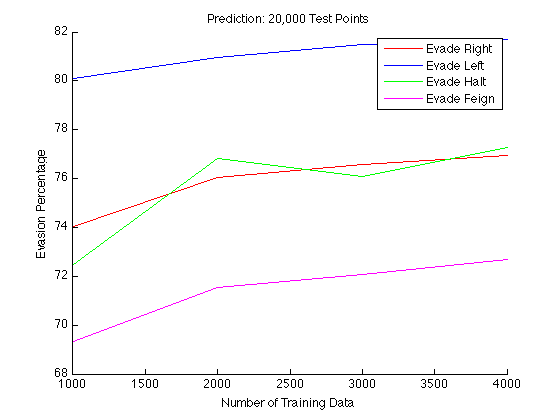
\includegraphics[width = 7.5 cm]{evadeFigures/prediction}
		\label{evade:prediction}}
	\subfigure[]{
		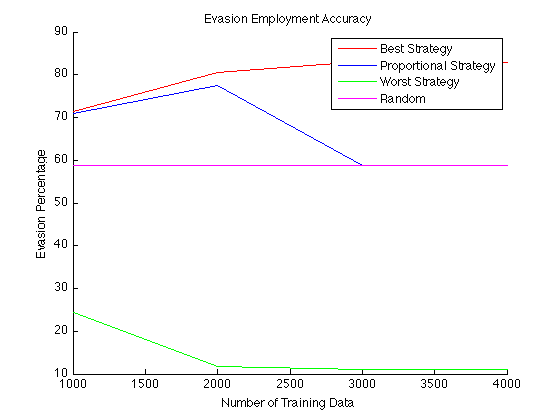
\includegraphics[width = 7.5 cm]{evadeFigures/overallAccuracy}
		\label{evade:accuracy}}
	\subfigure[]{
		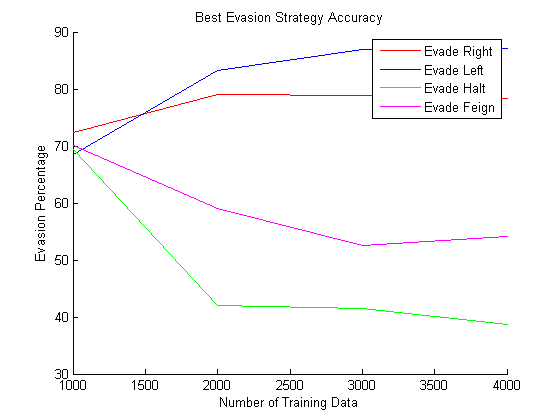
\includegraphics[width = 7.5 cm]{evadeFigures/bestAccuracy}
		\label{evade:bestAccuracy}}
	\subfigure[]{
		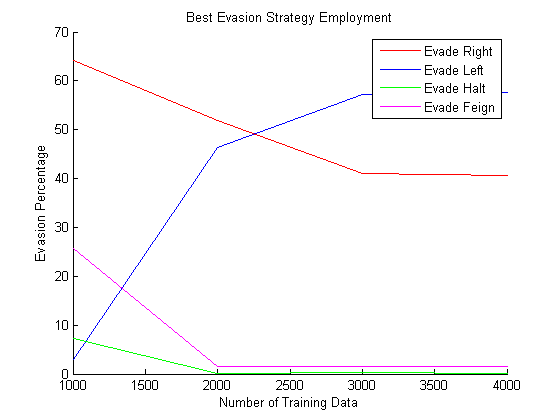
\includegraphics[width = 7.5 cm]{evadeFigures/bestEmployment}
		\label{evade:bestEmployment}}
\caption{SVM Evasion Testing Results.}
\label{evade:all}
\end{figure}

Ultimately, we are interested in the evasion accuracy based on the employment of the SVM predictions. Using probability SVM models\cite{libsvm}, three different employment agents were designed: one to employ the best evasion strategy, one to employ an evasion strategy sampled from a proportional distribution (weighted by the probability returned by the SVM), and one to employ the worst evasion strategy, each according to the probability estimates provided by the SVMs. These agents were then tested against all opponents for 10,000 battles. Results from these tests are shown in Figure \ref{evade:all}\subref{evade:accuracy}.

As expected, choosing the best evasion strategy according to the SVM probability estimates leads to an evasion percentage of over 80\%, whereas choosing the worst evasion strategy leads to the agent being hit by approximately 90\% of the bullets. For all strategies, as the number of training examples increases, the performance begins to approach an asymptotic evasion percentage, suggesting that employment performance does not change as training examples continue to increase. This is to be expected due to the nature that each enemy agent will ultimately target their opponent in a different manner, thus leading to models not being capable of capturing every form of targeting.

To understand what has been learned by the evasion SVMs, we must look closer into the employment of each individual evasion strategy. As depicted by Figure \ref{evade:all}\subref{evade:bestAccuracy}, we find that as the number of training examples increases, evading via halting or feigning seems to decrease in performance, while evading via movement to the left or right seems to increase. This is somewhat concerning, as we saw earlier that employing the best strategy leads to asymptotically increasing evasion performance. However, if we turn our attention to the employment percentage of each strategy, depicted in Figure \ref{evade:all}\subref{evade:bestEmployment}, we find that as the number of training examples increases, dodging left/right are used more often than halt and feign. Thus, we see that the SVMs are learning that there are more situations in which evading by movement to the left/right is likely to be successful compared to evading by halting or feigning.

By visual inspection, we have found that dodging left/right is typically employed to avoid placing the agent close to a wall. If there is a wall directly towards the left direction, the agent will typically choose to evade to the right, and vice versa. Similarly, feign is typically employed when the agent gets caught in a corner, a position which occurs infrequently (thus the low employment percentage of the strategy) and often ends in being hit by a bullet (thus the low evasion accuracy when feign is employed). Lastly, we typically only see halt employed when the agent is far away and both agents are in motion. Even then, halt is scarcely chosen as it is a rather ineffective evasion movement.

\subsection*{Targeting Results}
\subsubsection*{SVM Targeting}
In order to gather training data for the targeting SVM, the agent's cannon was constantly kept aligned towards the enemy. The enemy was then fired upon by randomly picking one of the 21 different firing angles, firing according to this angle, and using the firing angle as an additional feature. An SVM model was then trained using an RBF kernel with a 5-fold cross validation grid search to optimize the hyper-parameters (slack penalty and kernel bandwidth). Two different subsets of training data were collected: data when battling an agent using the evasion SVMs, and another set when battling all enemy agents. Overall, eight models were trained using differing numbers of training points. A test data set, comprised of 100,000 data points collected from battles against all enemy agents, was used to test the SVMs for prediction accuracy, as depicted in Figure \ref{target:all}\subref{target:prediction}. As the number of training data points increases, so does the accuracy of the SVMs. However, the accuracy stabilizes as the number of training data points increases. Furthermore, training by collecting data from multiple agents provided better models for prediction. 

As was the case with the evasion SVMs, we are interested in the accuracy of employing these predictions. Using probability SVM models trained on all enemy agents, testing data was collected by firing at the multiple opponents for 1,000 battles whenever their was a greater than 60\% chance of hitting the enemy. This data was then separated to observe the accuracy of hitting the enemy at differing thresholds, as depicted in Figure \ref{target:all}\subref{target:accuracy}. We can see from this chart that as the probability threshold increases, so does the accuracy of hitting the enemy. Furthermore, the more data used to train the SVM model, the higher the accuracy. 

\begin{figure}[h]
	\centering
	\subfigure[]{
		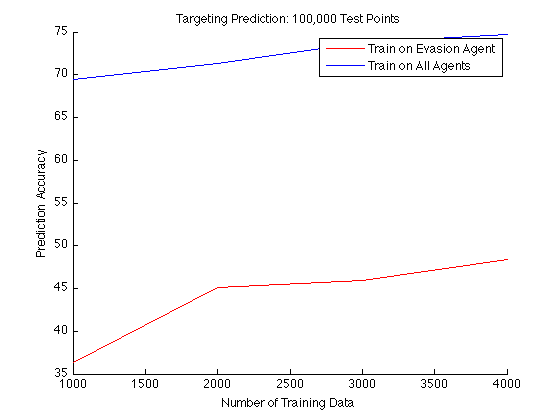
\includegraphics[width = 7.5 cm]{targetFigures/prediction}
		\label{target:prediction}}
	\subfigure[]{
		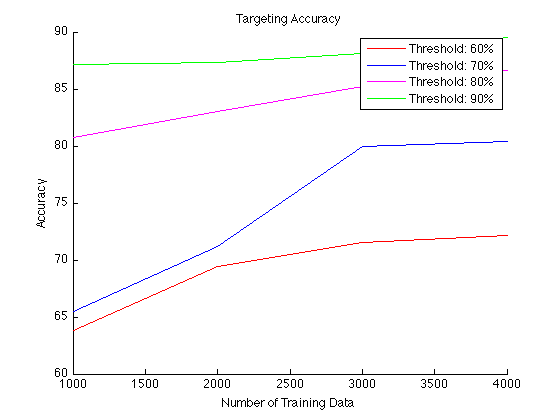
\includegraphics[width = 7.5 cm]{targetFigures/accuracy}
		\label{target:accuracy}}
	\subfigure[]{
		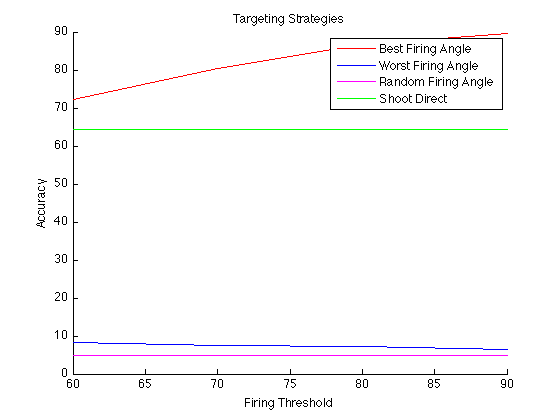
\includegraphics[width = 7.5 cm]{targetFigures/strategies}
		\label{target:strategies}}
\caption{SVM Targeting Testing Results}
\label{target:all}
\end{figure}

Lastly, we looked at these results compared with different firing strategies. In the chart below, an SVM model was trained from 4,000 data points drawn from the differeing opponents. The accuracy from the best firing angle according to the SVM is compared with the accuracy from the worst firing angle. These results are shown in Figure \ref{target:all}\subref{target:strategies}. As expected, choosing the worst firing angle has an extremely low targeting accuracy when compared with employing the best firing angle. As a benchmark, the accuracy of shooting directly at the opponent, as well as shooting at a random firing angle is shown. Overall, our SVM model is able to perform better at targeting the opponent than these other strategies, and we are capable of achieving ~90\% accuracy using these SVM models. 

From observing this targeting scheme, it appears the SVM models have learned that the best time to fire at an opponent is when they are near by, or close to a corner / wall. When the enemy is near a wall / corner, the firing angle is often times chosen such that it will strike the enemy if they move away from the wall, or if they do nothing. Thus, similar to the evasion strategies that were learned, proximity to walls and corners plays a large part in an enemy being hit by fired bullets. 

\subsubsection*{RL Targeting}
We found that Q-learning responds best when we slowly increase the difficulty of a targeting scheme rather than just throwing the system off the deep-end by pitting it against the best enemy agents. We started by training the agent against an enemy that sits stationary without firing back. The agent was able to learn that it should always fire straight ahead, achieving an accuracy of 100\%. We then increased the difficulty to an opponent that moves with a uniform velocity in a linear path around the battlefield. After 100 000 rounds, an accuracy of 50\% was achieved. After this we could begin to train the agent against complex opponents. We trained the agent for over 1 million rounds against a version of a top-ranking robot that doesn't shoot back. Agents that do not fire back help prolong the training by prolonging each rounds length.
\begin{figure}[h]
	\centering
		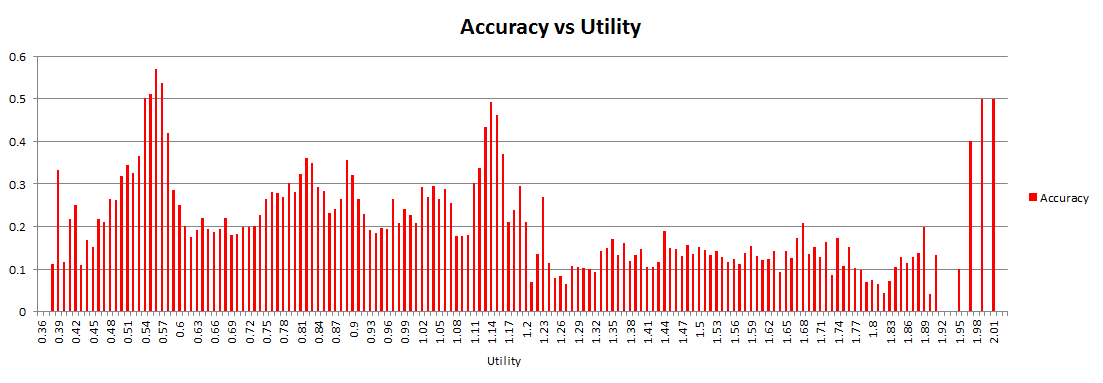
\includegraphics[width=15 cm]{Q_accu.png}
	\caption{A distribution of accuracy versus the utility value for 1048576 test cases}
	\label{q_accu}
\end{figure}
We then tested our agent against this opponent. Our agent uses a greedy policy arbiter that fires at the angle with the highest $Q$ value. If that value is below a threshold, then the agent does not fire. Although the $Q$ value captures more than just the likelihood of hitting the opponent, we expected a high correlation between the $Q$ value and accuracy of the shot. However, as seen in Figure \ref{q_accu}, that is not the case. We believe this happens because the linear function learned does not capture the intricacies of the environment. This is evident in the fact that the Q-learning agent is able to win only 2\% of the rounds against this opponent, who doesn't even fire back. At the time of writing this report, we feel that if we run training for many more cycles we might see improvements, however it is reasonable to question whether a linear approximation method can possibly capture the true nature of the system and if so, whether the number of training cycles required are tractable. Another area that could be looked into is the possibility that designing more complex features might help the performance.

\subsection*{Integrated Performance}
Using the best SVM evasion models as well as the best SVM targeting model (according to the test accuracy), an integrated agent was created to apply both of the targeting and evasion techniques simultaneously. Using this integrated agent, 100 battles against each of the opponents were ran, for a total of 1,000 battles. Table \ref{svm_thresh} depicts the results of these battles utilizing different thresholds for targeting the enemy. As the table shows, the win percentage increases until the threshold is set above 70\%, at which point the win percentage begins to drop. Overall, we have achieved a success rate of approximately 42\% when implementing SVMs to target and evade against some of the more competitive hand-written Robocode agents. 

\begin{table}[h]
\centering
    \begin{tabular}{|c|c|}
        \hline
        \bf{Threshold} & \bf{Overall Wins (\%) }\\ \hline
        50\%      & 38.8   \\ \hline
        60\%      & 39.3   \\ \hline
        70\%      & 42.2   \\ \hline
        80\%      & 33.4   \\ \hline
        90\%      & 23.9   \\
        \hline
    \end{tabular}
\label{svm_thresh}
\caption{A comparison of overall performance and the threshold used for targeting.}
\end{table}

\section{Conclusion}
We have designed agents that are able to learn and successfully employ evasion and targeting strategies using support vector machines. The fact that an integrated agent which combines the learned strategies is able to win 42.2\% of the battles shows that our performance is competitive against some of the best robots written by humans. 

Compared to the SVM-targeting agent, our approach using reinforcement learning was less successful. Though we were able to achieve good accuracy against very simple robots, the agent was not able to learn an efficient targeting strategy against more complex opponents, even after a large number of rounds. We attribute this to two factors. First, we use a linear approximation for the $Q$ function, whereas SVMs use a more flexible RBF kernel. Second, it is easy to do a grid-search
combined with cross-validation to choose the best hyperparameters for an SVM; it is much harder to tweak the constants in Q-learning. 

Our main focus for future work would be improving the running time of the SVM-targeting agent, along with trying to improve the performance of the Q-learning agent through more complex features.

\bibliographystyle{IEEEtranS}
\bibliography{sources}

\end{document}


\def\therefore{\boldsymbol{\text{ }
\leavevmode
\lower0.4ex\hbox{$\cdot$}
\kern-.5em\raise0.7ex\hbox{$\cdot$}
\kern-0.55em\lower0.4ex\hbox{$\cdot$}
\thinspace\text{ }}}
